\documentclass[11pt,a4paper]{article}
\usepackage[margin=25mm,top=22mm,bottom=23mm]{geometry}
\usepackage{amsmath,amssymb,amsthm,booktabs,mathtools,xcolor,microtype,tikz}
\usepackage[colorlinks=true,urlcolor=teal!65!black,linkcolor=teal!65!black,citecolor=teal!65!black]{hyperref}
\usepackage{fancyhdr}
\pagestyle{fancy}\fancyhf{}\fancyhead[L]{\small Real entanglement witnesses under local filters}\fancyhead[R]{\small Anonymous}\fancyfoot[C]{\thepage}
\setlength{\headheight}{15pt}\setlength{\emergencystretch}{2em}
\newtheorem{theorem}{Theorem}\newtheorem{lemma}[theorem]{Lemma}\newtheorem{prop}[theorem]{Proposition}\newtheorem{cor}[theorem]{Corollary}
\theoremstyle{definition}\newtheorem{definition}[theorem]{Definition}\newtheorem*{conj}{Conjecture 9 of Shen, Chen and Bian}\newtheorem{remark}[theorem]{Remark}
\newcommand{\tr}{\operatorname{tr}}\newcommand{\im}{\operatorname{Im}}\newcommand{\adj}{\operatorname{adj}}\newcommand{\id}{\mathbb I}
\newcommand{\eps}{\varepsilon}\newcommand{\ket}[1]{\lvert #1\rangle}\newcommand{\bra}[1]{\langle #1\rvert}\newcommand{\F}{\mathrm F}\newcommand{\op}{\mathrm{op}}\newcommand{\C}{\mathbb C}
\newcommand{\cB}{\mathcal B}\newcommand{\cR}{\mathcal R}\newcommand{\vecm}{\mathrm{vec}}
\title{\bfseries Two-qutrit entanglement invisible to real witnesses under every local filter}
\author{Anonymous\\[3pt]{\small DOI \href{https://doi.org/10.5281/zenodo.24540619}{10.5281/zenodo.24540619}}}\date{24 November 2026}
\begin{document}
\maketitle
\begin{abstract}
An entanglement witness is an observable whose expectation is nonnegative on every separable state and negative on some entangled state. Shen, Chen and Bian conjectured that witnesses written with real matrices lose nothing, provided each laboratory may first change its local basis (Conjecture~9(i)) or apply an invertible local filter (Conjecture~9(ii)). We disprove both parts. We give an explicit full-rank two-qutrit state, with positive-definite partial transpose, that a complex witness detects while every real witness, after any invertible local filters and in any limit of such operations, has strictly positive expectation on it; the same holds on an open ball of states. Part~(i) already fails for a qubit and a ququart, the smallest dimension in which it can fail. More generally, in every dimension the conjecture holds exactly when every exposed point of the set of normalised block-positive operators is a limit of filtered real ones, and when it fails it fails on an open set of full-rank states. A polynomial invariant decides which members of an exposed family of Ha and Kye have real representatives. One local ancilla qubit restores detection, and so does a second copy of the state used as an ancilla.
\end{abstract}

\section{Introduction}
This section states the problem, explains why it matters, summarises what was known, lists what is new and gives a roadmap.

\paragraph{The problem.}
Entanglement is the correlation between quantum systems that cannot be produced by local operations and shared randomness. The standard way to certify it in a laboratory is an \emph{entanglement witness}: a Hermitian observable $V$ with $\tr(V\sigma)\geq0$ for every separable state $\sigma$ and $\tr(V\rho)<0$ for some entangled state $\rho$ \cite{horodecki,guhne}. Every entangled state is detected by some witness \cite{horodecki}. A witness is a matrix in a chosen product basis, and in general its entries are complex. Shen, Chen and Bian asked how much is lost if only witnesses with \emph{real} matrix entries are used \cite{shen}. Without any freedom of basis the loss is real: the state $(\ket{00}+i\ket{11})/\sqrt2$ has a separable real part and is detected by no real witness \cite[Section III]{shen}. They therefore allowed each laboratory to move to a better local basis first. In their terms, $E^{\mathrm{LU}}$ is the set of witnesses $(U\otimes V)R(U\otimes V)^\dagger$ with $R$ a real witness and $U,V$ unitary, and $E^{\mathrm{SLOCC}}$ is the larger set obtained when $U,V$ are only required to be invertible \cite[Definition~1]{shen}.

\begin{conj}[{\cite[Conjecture 9]{shen}}]
(i) Every bipartite entangled state is detected by some witness in $E^{\mathrm{LU}}$. (ii) More generally, every bipartite entangled state is detected by some witness in $E^{\mathrm{SLOCC}}$.
\end{conj}
Part (i) implies part (ii), so a counterexample to (ii) is also a counterexample to (i).

\paragraph{Why it matters.}
Real and complex quantum theory make different predictions in network experiments \cite{renou}, and the imaginary parts of density matrices have been studied as a resource of their own \cite{hickey}. The conjecture asks a sharper operational question: whether the complex phases needed for an entanglement test can always be moved out of the observable and into the choice of local basis or local filter. If they could, every entanglement test could be carried out with real-matrix observables after a suitable local preprocessing. Local filters are also the operations that define the SLOCC classification of entangled states, so the question concerns a natural symmetry class of witnesses.

\paragraph{What was known.}
Shen, Chen and Bian proved part (i) whenever the partial transpose of the state has a negative eigenvalue \cite[Lemma 10(i)]{shen}. Because $2\times2$ and $2\times3$ states with positive partial transpose (PPT) are separable \cite{horodecki}, the conjecture holds in total dimension below eight. For two qutrits they proved part (i) for the PPT entangled states built from unextendible product bases and part (ii) for all PPT entangled states of rank four \cite[Theorem 11]{shen}. Their Example~12 is a $4\times4$ PPT entangled state that no real witness detects in the given basis but a locally rotated real witness does. A counterexample therefore has to be a PPT entangled state whose real part remains separable after every local filtering \cite[Lemma 10(ii) and its SLOCC version]{shen}. Skowronek had shown that no \emph{finite} family of positive maps, combined with arbitrary local filters, detects all two-qutrit entanglement, using the same Ha--Kye family of maps \cite{skowronek}; the real witnesses form an infinite family, so his result does not settle the question.

\paragraph{What is new.}
\begin{itemize}
\item \emph{A two-qutrit counterexample to both parts} (Theorem~\ref{thm:one}). An explicit full-rank PPT entangled state is detected by a complex witness, while every filtered real witness and every limit of such witnesses has expectation above $8.5\times10^{-10}$ on it. The same holds on a ball of Frobenius radius $8\times10^{-10}$.
\item \emph{Part (i) fails in the smallest possible dimension} (Theorem~\ref{thm:2x4}). On $\C^2\otimes\C^4$ there are full-rank PPT entangled states detected by a filtered real witness but by no witness in $E^{\mathrm{LU}}$. So $E^{\mathrm{LU}}$ and $E^{\mathrm{SLOCC}}$ differ in detection power; whether part (ii) fails there is open.
\item \emph{A general criterion} (Theorem~\ref{thm:dichotomy}). In every dimension, part (ii) holds exactly when every exposed point of the set of trace-one block-positive operators is a limit of filtered real ones (equivalently, every extreme point is); the same holds for part (i) with local unitaries. Whenever the conjecture fails, it fails on an open set of full-rank PPT entangled states.
\item \emph{A classification on an exposed family} (Theorem~\ref{thm:class}). A degree-nine polynomial invariant decides exactly which witnesses in the exposed Ha--Kye family \cite{hakye} have filtered real representatives.
\item \emph{What restores detection} (Section~\ref{sec:copy}). One local ancilla qubit in a real pure state restores detection under local unitaries. A second copy of the state can serve as that ancilla when invertible filters are allowed.
\end{itemize}
The witness and the separable state that underlie the counterexample are not new: both are due to Ha and Kye \cite{hakye,hk12}. The new ingredients are the observation that exposedness converts any witness outside the filtered real class into an open set of missed states, the polynomial invariants that place a specific exposed witness outside that class, and an exact finite certificate for the constants.

\paragraph{Roadmap.}
Section~\ref{sec:setting} fixes notation and definitions and compares the filtered real class with the sets of the conjecture. Section~\ref{sec:dichotomy} proves the general criterion. Section~\ref{sec:example} constructs the two-qutrit counterexample and the invariant that separates it from the filtered real class. Section~\ref{sec:class} classifies the Ha--Kye family. Section~\ref{sec:bounds} proves the explicit constants. Section~\ref{sec:2x4} treats the qubit--ququart case. Section~\ref{sec:copy} discusses ancillas and copies, and Section~\ref{sec:scope} collects limitations and open problems.

\section{Setting and definitions}\label{sec:setting}
This section fixes the notation, recalls the convex geometry of witnesses and states precisely which class of operators the results exclude.

We work on $\C^m\otimes\C^n$ with the ordered product basis $\ket{ij}$, the first index changing slowly; most of the paper has $m=n=3$ and $i,j\in\{0,1,2\}$. For a matrix $X$, $\bar X$ is the entrywise complex conjugate, $X^T$ the transpose and $X^\Gamma$ the partial transpose on the second factor, $(X^\Gamma)_{ij,kl}=X_{il,kj}$. Partial transposition on the first factor is written $X^{\Gamma_A}$. Both are isometries for the Frobenius norm $\|X\|_\F=(\tr X^\dagger X)^{1/2}$, and $X^{\Gamma_A}=(X^\Gamma)^T$, so they also have the same operator norm $\|\cdot\|_\op$ (largest singular value). States are paired with operators by the ordinary trace $\tr(V\rho)$. $E_{ij}=\ket i\bra j$ denotes a matrix unit, $\lambda_{\min}$ the smallest eigenvalue, and the \emph{relative interior} of a convex set is its interior within its own affine hull.

\begin{definition}[Block positivity, witnesses, Choi matrices]
A Hermitian $V$ is \emph{block-positive} if $\bra{xy}V\ket{xy}\geq0$ for all product vectors $x\otimes y$. A block-positive operator with a negative eigenvalue is an \emph{entanglement witness}. A linear map $\Phi:M_m\to M_n$ has \emph{Choi matrix} $C_\Phi=\sum_{i,j}E_{ij}\otimes\Phi(E_{ij})$; $\Phi$ is positive exactly when $C_\Phi$ is block-positive. A positive map, or its witness, is \emph{decomposable} if it is a sum of a completely positive map and a completely positive map composed with the transpose, that is $V=P+Q^\Gamma$ with $P,Q\succeq0$; otherwise it is \emph{indecomposable}. Only indecomposable witnesses detect PPT entangled states.
\end{definition}

Let $\cB$ be the set of trace-one block-positive operators on $\C^m\otimes\C^n$. Every nonzero block-positive $V$ has $\|V\|_\F\leq\tr V$: Gurvits and Barnum proved that $\id+\Delta$ is separable whenever $\|\Delta\|_\F\leq1$ \cite[Theorem 1]{gurvits}, and testing $V$ on $\id-V/\|V\|_\F$ gives the inequality. (Their theorem is stated for $N\times N$ systems; a block-positive operator on $\C^m\otimes\C^n$ extends by zero to one on $\C^N\otimes\C^N$, $N=\max(m,n)$, with the same trace and norm.) Hence $\cB$ is compact.

\begin{definition}[Faces and exposure]
A point $E$ of a compact convex set $K$ is \emph{extreme} if it is not a proper convex combination of two other points of $K$, and \emph{exposed} if some linear functional attains its maximum on $K$ at $E$ and nowhere else. Every exposed point is extreme. For $\cB$, $E$ is exposed exactly when there is a separable operator $D\succeq0$ with $\tr(DE)=0$ and $\tr(DV)>0$ for every other $V\in\cB$; we then say that $D$ \emph{exposes} $E$. (Given an exposing functional $\ell$ with maximum $\ell(E)$ on the hyperplane $\tr V=1$, write $\ell(V)=\tr(YV)$ and put $D=\ell(E)\id-Y$; then $\tr(DV)\geq0$ on all block-positive $V$, which means that $D$ is separable \cite{horodecki}.) In the language of positive maps, the ray through $E$ is then an exposed face of the cone of positive maps, and the set of separable states with zero pairing is its \emph{dual face} \cite{hakye}.
\end{definition}

\begin{definition}[Filtered real and locally unitary real operators]
A \emph{local filter} is $K=A\otimes B$ with $A\in GL(m,\C)$ and $B\in GL(n,\C)$. An operator is \emph{filtered real} if it equals $KRK^\dagger$ with $K$ a local filter and $R$ real symmetric in the product basis, and \emph{locally unitary real} if moreover $A$ and $B$ are unitary. Let $\cR$ (respectively $\cR_{\mathrm U}$) be the closure of the set of filtered real (respectively locally unitary real) members of $\cB$.
\end{definition}

Congruence by a local filter preserves block positivity in both directions, and by Sylvester's law of inertia it preserves the existence of a negative eigenvalue. Hence the filtered real witnesses are exactly the set $E^{\mathrm{SLOCC}}$ of the conjecture, and the locally unitary real witnesses are exactly $E^{\mathrm{LU}}$. A filtered real block-positive operator without a negative eigenvalue is positive semidefinite and detects nothing. So a state is detected by $E^{\mathrm{SLOCC}}$ if and only if some element of $\cR$ has negative expectation on it: one direction is immediate, and for the other a negative expectation persists along an approximating sequence. A filter can be rescaled to a contraction, which is a physical success branch of a local operation, without changing the sign of any expectation.

Figure~\ref{fig:cone} shows the geometry behind the whole paper.
\begin{figure}[t]
\centering
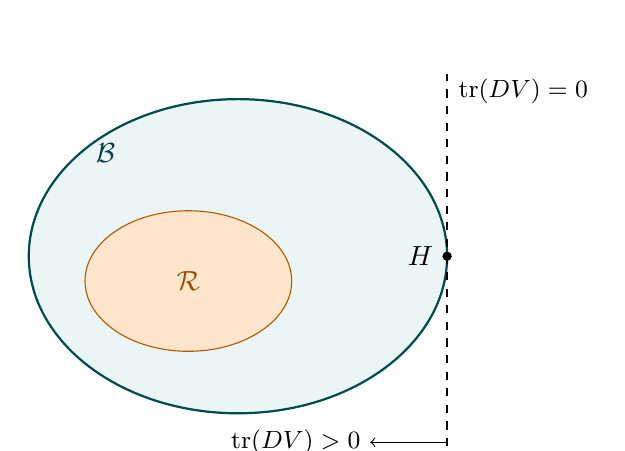
\begin{tikzpicture}[scale=1.05]
 \fill[teal!8] (2.8,0.8) ellipse (2.53 and 1.9);
 \draw[teal!60!black,thick] (2.8,0.8) ellipse (2.53 and 1.9);
 \fill[orange!20] (2.2,0.5) ellipse (1.25 and 0.85);
 \draw[orange!70!black] (2.2,0.5) ellipse (1.25 and 0.85);
 \node[orange!60!black] at (2.2,0.5) {$\mathcal R$};
 \node[teal!50!black] at (1.2,2.05) {$\mathcal B$};
 \fill (5.33,0.8) circle (1.6pt);
 \node[left] at (5.28,0.8) {$H$};
 \draw[thick,dashed] (5.33,-1.7) -- (5.33,3.0);
 \node[right] at (5.35,2.8) {\small $\tr(DV)=0$};
 \draw[->] (5.33,-1.45) -- (4.4,-1.45);
 \node[left] at (4.4,-1.45) {\small $\tr(DV)>0$};
\end{tikzpicture}
\caption{Schematic of the trace-one slice. $\cB$ is the convex set of trace-one block-positive operators and $\cR\subset\cB$ the closure of its filtered real members. A separable $D$ exposes the witness $H$: the hyperplane $\tr(DV)=0$ touches $\cB$ only at $H$. If $H\notin\cR$, the compact set $\cR$ keeps a positive distance from that hyperplane, so slightly moving $D$ towards entanglement yields states that $H$ detects and $\cR$ does not.}\label{fig:cone}
\end{figure}

\section{Exposed witnesses decide the conjecture}\label{sec:dichotomy}
This section proves that the conjecture, in any fixed dimension, is decided by the exposed points of $\cB$, and that every failure is robust.

\begin{lemma}\label{lem:exposed}
Let a separable $D\succeq0$ expose $H\in\cB$, and suppose $H\notin\cR$. Then $g:=\min_{V\in\cR}\tr(DV)>0$. If moreover $D\succ0$ and $D^\Gamma\succ0$, then for every $0<\eps<\min\{g,\lambda_{\min}(D),\lambda_{\min}(D^\Gamma)\}$ the state $\rho_\eps=(D-\eps\id)/\tr(D-\eps\id)$ is a full-rank PPT entangled state on which $H$ is negative and every element of $\cR$ is positive. These properties persist on a Frobenius neighbourhood of $\rho_\eps$ in the trace-one Hermitian matrices. The same statements hold with $\cR_{\mathrm U}$ in place of $\cR$.
\end{lemma}
\begin{proof}
The pairing $V\mapsto\tr(DV)$ is continuous and $\cR$ is compact, so the minimum is attained. It is positive because the only zero of the pairing on $\cB$ is $H$, which is not in $\cR$. For trace-one $V$, $\tr\bigl(V(D-\eps\id)\bigr)=\tr(DV)-\eps$. This is $-\eps<0$ at $V=H$ and at least $g-\eps>0$ on $\cR$. The bounds on $\eps$ make $D-\eps\id$ and its partial transpose $D^\Gamma-\eps\id$ positive definite; negativity of the block-positive $H$ certifies entanglement. All conditions are strict inequalities between continuous functions, and $|\tr(V\xi)|\leq\|V\|_\F\|\xi\|_\F\leq\|\xi\|_\F$ uniformly on $\cB$ for every perturbation $\xi$, so they survive small perturbations.
\end{proof}
Ha and Kye observed that an exposed indecomposable witness detects an open set of PPT states \cite[Introduction]{hakye}; Lemma~\ref{lem:exposed} is the same mechanism applied to the compact class $\cR$.

\begin{lemma}\label{lem:fullrank}
Let $D$ expose a point $H\in\cB\setminus\cR_{\mathrm U}$. Then $D\succ0$ and $D^\Gamma\succ0$.
\end{lemma}
\begin{proof}
If $Dv=0$ for some unit vector $v$, then $\ket v\bra v\in\cB$ has zero pairing with $D$, so it equals $H$. By the Schmidt decomposition a local unitary turns $v$ into a real vector, so $\ket v\bra v\in\cR_{\mathrm U}$, a contradiction. If $D^\Gamma v=0$, then $(\ket v\bra v)^\Gamma$ is block-positive with trace one and $\tr\bigl(D(\ket v\bra v)^\Gamma\bigr)=\tr(D^\Gamma\ket v\bra v)=0$, so it equals $H$. Writing $v=(U\otimes U')w$ with $w$ real gives $(\ket v\bra v)^\Gamma=(U\otimes\bar U')(\ket w\bra w)^\Gamma(U\otimes\bar U')^\dagger$, again in $\cR_{\mathrm U}$.
\end{proof}
Since $\cR_{\mathrm U}\subseteq\cR$, the lemma applies in particular to exposed points outside $\cR$.

\begin{theorem}[When the conjecture holds]\label{thm:dichotomy}
Fix $m,n\geq2$. The following are equivalent:
\begin{enumerate}
\item[(a)] every entangled state on $\C^m\otimes\C^n$ is detected by a witness in $E^{\mathrm{SLOCC}}$;
\item[(b)] every extreme point of $\cB$ lies in $\cR$;
\item[(c)] every exposed point of $\cB$ lies in $\cR$.
\end{enumerate}
If they fail, the entangled states missed by $E^{\mathrm{SLOCC}}$ include an open set of full-rank PPT states. The same equivalences hold for $E^{\mathrm{LU}}$ with $\cR_{\mathrm U}$ in place of $\cR$.
\end{theorem}
\begin{proof}
(b)$\Rightarrow$(a). An entangled $\rho$ has $\tr(V\rho)<0$ for some $V\in\cB$ \cite{horodecki}. By Minkowski's theorem $V$ is a convex combination of extreme points of $\cB$, so one of them, $Z$, has $\tr(Z\rho)<0$. By (b), $Z$ is a limit of filtered real members of $\cB$, and those close enough to $Z$ are negative on $\rho$; such an operator is block-positive and not positive semidefinite, hence a witness in $E^{\mathrm{SLOCC}}$.

(a)$\Rightarrow$(c). If an exposed point $H$ lies outside $\cR$, Lemma~\ref{lem:fullrank} shows that its exposing operator $D$ satisfies $D\succ0$ and $D^\Gamma\succ0$, and Lemma~\ref{lem:exposed} produces an open set of full-rank PPT entangled states missed by $\cR$, hence by $E^{\mathrm{SLOCC}}$. This also proves the final assertion.

(c)$\Rightarrow$(b). Suppose an extreme point $Z$ of $\cB$ lies outside $\cR$. The convex hull $\mathcal C$ of the compact set $\cR$ is compact, and $Z\notin\mathcal C$, because a representation of $Z$ as a convex combination of points of $\cR\subseteq\cB$ would force all of them to equal $Z$. Choose a Hermitian $Y$ with $\tr(YZ)>c:=\max_{\mathcal C}\tr(Y\,\cdot\,)$, and let $Y_0$ be its traceless part, which is nonzero. Put $M=\max_{\cB}\tr(Y\,\cdot\,)\geq\tr(YZ)>c$ and let $d_{\cB}$ be the Frobenius diameter of $\cB$. Fix $X_0\in\cB$ and, for $s>0$, put $a_s=X_0-sY_0$. For $V\in\cB$,
\[
 \|V-a_s\|_\F^2=\|V-X_0\|_\F^2+2s\tr\bigl(Y_0(V-X_0)\bigr)+s^2\|Y_0\|_\F^2 ,
\]
and on $\cB$ the functional $\tr(Y_0V)$ differs from $\tr(YV)$ by a constant. Let $V_s$ be a point of $\cB$ farthest from $a_s$. Comparing with a maximiser of $\tr(Y\,\cdot\,)$ gives $\tr(YV_s)\geq M-d_{\cB}^2/(2s)$, which exceeds $c$ once $s>d_{\cB}^2/(2(M-c))$; then $V_s\notin\cR$. Finally $V_s$ is exposed: $\cB$ lies in the ball of radius $\|V_s-a_s\|_\F$ about $a_s$, and if $V\in\cB$ satisfies $\tr\bigl((V_s-a_s)(V-V_s)\bigr)\geq0$ then
$\|V-V_s\|_\F^2=\|V-a_s\|_\F^2-\|V_s-a_s\|_\F^2-2\tr\bigl((V_s-a_s)(V-V_s)\bigr)\leq0$. So the functional $\tr\bigl((V_s-a_s)\,\cdot\,\bigr)$ is maximised on $\cB$ only at $V_s$. This contradicts (c).

The argument for $E^{\mathrm{LU}}$ is identical.
\end{proof}

The extreme points of $\cB$ that are positive semidefinite are pure states $\ket v\bra v$, which lie in $\cR_{\mathrm U}$ by the Schmidt decomposition; so conditions (b) and (c) concern only extreme points that are witnesses. Theorem~\ref{thm:dichotomy} reduces each instance of the conjecture to a question about single operators: to refute it, exhibit one exposed witness outside $\cR$. The next section does this for two qutrits.

\section{The two-qutrit counterexample}\label{sec:example}
This section writes down the witness, its exposing separable operator and a polynomial invariant that separates the witness from the filtered real class, and states the main theorem.

\paragraph{The data.}
For real $a,b,c$ and complex $u$ let $T(a,b,c;u)$ be the Hermitian $9\times9$ matrix with diagonal entry $(a,b,c)_{(j-i)\bmod3}$ at $\ket{ij}$, entry $u$ in row $\ket{ii}$ and column $\ket{i+1,i+1}$, entry $\bar u$ in the transposed position (indices mod $3$), and zeros elsewhere. Set
\begin{align}
 W&=T(3,1,4;-4-3i),  &D&=T\bigl(48,48,24;(144+48i)/5\bigr),\label{eq:data}\\
 H&=W/24, &\rho_\eps&=\frac{D-\eps\id}{360-9\eps}.\label{eq:state}
\end{align}
Ha and Kye studied the maps $\Phi[a,b,c;\theta]$ on $M_3$ with Choi matrix
\begin{multline*}
 \sum_{k}\bigl(a E_{kk}\otimes E_{kk}+c\,E_{kk}\otimes E_{k+1,k+1}+b\,E_{kk}\otimes E_{k+2,k+2}\bigr)\\
 -\sum_{k}\bigl(e^{i\theta}E_{k,k+1}\otimes E_{k,k+1}+e^{-i\theta}E_{k+1,k}\otimes E_{k+1,k}\bigr),
\end{multline*}
indices mod 3 \cite{hakye,hk12}. They proved that $\Phi[a,b,c;\theta]$ is positive if and only if $a+b+c\geq p_\theta$ and, when $a\leq1$, $bc\geq(1-a)^2$, where $p_\theta=2\max_{k}\cos(\theta+2\pi k/3)$ \cite[Theorem 2.2]{hk12}. On the boundary curve
\begin{equation}\label{eq:family}
 a(t)=1-\frac{(p_\theta-1)t}{1-t+t^2},\qquad b(t)=\frac{(p_\theta-1)t^2}{1-t+t^2},\qquad c(t)=\frac{p_\theta-1}{1-t+t^2},\qquad t>0,
\end{equation}
$\Phi_\theta(t)=\Phi[a(t),b(t),c(t);\theta]$ is indecomposable \cite{hk12} and exposed \cite[Theorem 3.2]{hakye} unless $\theta=(2k-1)\pi/3$ or $(\theta,t)=(2k\pi/3,1)$, $k\in\mathbb Z$. Take $e^{i\theta}=(4+3i)/5$ and $t=2$. Then $|\theta|<\pi/3$, $p_\theta=2\cos\theta=8/5$ and $(a,b,c)=(3/5,4/5,1/5)$, which satisfy both positivity conditions with equality; $W$ is five times the Choi matrix of $\Phi_\theta(2)$. Ha and Kye also exhibited a separable operator $\varrho_0(\theta,t)$ in the relative interior of the dual face \cite[Section 4]{hakye}. Their pairing transposes the state, so with the ordinary trace the exposing operator is the transpose; $D=16\,\varrho_0(\theta,2)^T$. A point in the relative interior of the dual face of an exposed ray pairs to zero only with that ray, so $D$ exposes $H$ in the sense of Section~\ref{sec:setting}. Section~\ref{sec:bounds} gives a finite certificate of this exposure at our parameters that uses only the block positivity of $W$. The program \texttt{verify\_witness.py} rebuilds $W$ from the Ha--Kye map and $D$ from their product vectors and checks both identities exactly.

Diagonalising a three-dimensional circulant block and the two-dimensional blocks of the partial transpose gives
\begin{equation}\label{eq:ranks}
 \lambda_{\min}(D)=\frac{96-48\sqrt3}{5}>2,\qquad
 \lambda_{\min}(D^\Gamma)=36-\frac{12\sqrt{185}}5>3 .
\end{equation}
So $D/360$ is a separable state in the interior of the PPT set that lies on the boundary of the separable set, since $\tr(DW)=0$.

\paragraph{An invariant that vanishes on filtered real matrices.}
For $9\times9$ matrices $X,Y$ define the $9\times9$ matrix
\begin{equation}\label{eq:cov}
 C(X,Y)_{jb,ck}=\sum_{i,l=0}^2 X_{ij,kl}\,Y_{bl,ic},\qquad
 M(X)= C(X,\adj X),
\end{equation}
where $\adj X$ is the adjugate ($X\adj X=\det X\,\id$) and $jb$, $ck$ are ordered index pairs. On Hermitian matrices, $\chi(X)=\im\tr M(X)^3$ is a real polynomial of degree $27$. For invertible $X$ put $L(X)=C(X,X^{-1})$, so that $M(X)=(\det X)L(X)$ and, $\det X$ being real, $\chi(X)=(\det X)^3\im\tr L(X)^3$.

\begin{lemma}\label{lem:cov}
$\chi$ vanishes on every filtered real Hermitian matrix and on every limit of such matrices.
\end{lemma}
\begin{proof}
Let $K=A\otimes B$ and $S=B\otimes A^{-\dagger}$, where $A^{-\dagger}=(A^\dagger)^{-1}$. The adjugate obeys
$\adj(KXK^\dagger)=|\det K|^2 K^{-\dagger}(\adj X)K^{-1}$, first for invertible $X$ and then for all $X$ by continuity. In \eqref{eq:cov} the contracted indices $i$ cancel $A$ against $A^{-1}$ and the contracted indices $l$ cancel $\bar B$ against $B^{-\dagger}$. The four free indices give
$M(KXK^\dagger)=|\det K|^2 S M(X) S^{-1}$.
Hence $\chi(KXK^\dagger)=|\det K|^6\chi(X)$. For real $X$ the matrix $M(X)$ is real and $\chi(X)=0$. Since $\chi$ is a polynomial, it also vanishes on limits, whatever the condition numbers of the filters along the sequence.
\end{proof}
Exact arithmetic gives $\det W=-7040$ and
\begin{equation}\label{eq:chi}
 \tr M(W)^3=5\,007\,168\,700\,416+151\,720\,116\,387\,840\,i,\qquad
 \im\tr L(H)^3=-\frac{84\,184\,191}{193\,600}.
\end{equation}
The source of the imaginary part is visible by hand. The three kets $\ket{00},\ket{11},\ket{22}$ span a circulant block of $M(W)$ with diagonal $-3072$, forward entry $z=33024+17280i$ and reverse entry $\bar z/4$. The other six diagonal positions form three conjugate pairs whose cubic traces sum to a real number. Hence $\chi(W)=3(1-4^{-3})\im(z^3)$: it is nonzero because the cycle carries a complex phase and its two orientations have unequal weights.

\begin{theorem}\label{thm:one}
Let $\eps=1/160000$. Then $\rho_\eps$ is a full-rank PPT entangled two-qutrit state with $\tr(W\rho_\eps)=-8/19199997$. Every trace-one filtered real block-positive operator, and every limit of such operators, has expectation greater than $8.5\times10^{-10}$ on $\rho_\eps$. The same holds, with both signs preserved and the state remaining full-rank and PPT, for every trace-one Hermitian matrix within Frobenius distance $8\times10^{-10}$ of $\rho_\eps$. In particular both parts of Conjecture~9 fail for two qutrits.
\end{theorem}
Qualitatively, the theorem follows at once from Theorem~\ref{thm:dichotomy}: by \eqref{eq:chi} and Lemma~\ref{lem:cov}, $\chi(H)\neq0$, so the exposed point $H$ is not in $\cR$. Section~\ref{sec:bounds} proves the explicit constants.

The result concerns the matrix of a single witness on the given local spaces. An experiment may still reconstruct the state, or a complex witness, from several real measurement settings and signed classical postprocessing; Section~\ref{sec:copy} discusses what changes when the local spaces are enlarged.

\section{Which Ha--Kye witnesses have a real representative?}\label{sec:class}
This section shows that the counterexample is not an accident of the chosen parameters: a second invariant decides the question on the whole exposed Ha--Kye family.

In the diagonal ordering of $T$, the Choi matrix of $\Phi_\theta(t)$ is $T(a,c,b;u)$ with $u=-e^{i\theta}$ and $a,b,c$ from \eqref{eq:family}. To keep the formulas symmetric we rename the second and third diagonal weights, writing $\beta=c(t)=(p_\theta-1)/(1-t+t^2)$ and $\gamma=b(t)=(p_\theta-1)t^2/(1-t+t^2)$, so that the family is $T(a,\beta,\gamma;u)$.

\begin{theorem}\label{thm:class}
For the exposed members of the family, the following are equivalent: (1) $T(a,\beta,\gamma;u)$ lies in the closure of the filtered real Hermitian matrices; (2) it has a filtered real representative; (3) it has a locally unitary real representative; (4) $t=1$ or $\sin3\theta=0$. Every exposed ray that violates (4) yields an open set of full-rank PPT entangled states missed by every filtered real witness.
\end{theorem}
\begin{proof}
\emph{The invariant.} Take nine copies of $X_{ij,kl}$, labelled $0,\dots,8$. For each of the four index positions, contract the nine indices of that position against three Levi-Civita tensors (normalised by $\epsilon_{012}=1$) in the order given by the following ordered triples of copy labels, and sum over all index values; call the result $\Pi(X)$.
\[
\begin{array}{c|ccc}
\text{index position}&\multicolumn{3}{c}{\text{ordered triples of copy labels}}\\ \hline
 i\ (\text{row, first factor})&(0,1,2)&(3,4,5)&(6,7,8)\\
 j\ (\text{row, second factor})&(0,5,3)&(8,4,6)&(2,1,7)\\
 k\ (\text{column, first factor})&(1,2,6)&(5,0,7)&(8,4,3)\\
 l\ (\text{column, second factor})&(0,3,8)&(6,4,1)&(7,2,5)
\end{array}
\]
Under $X\mapsto KXK^\dagger$ each Levi-Civita contraction contributes a determinant, so $\Pi(KXK^\dagger)=(\det A)^3(\det B)^3(\overline{\det A})^3(\overline{\det B})^3\Pi(X)=|\det A\det B|^6\Pi(X)$, and $\Pi(\bar X)=\overline{\Pi(X)}$. Hence $\Pi$ is real on the closure of the filtered real matrices. Local unitary and SLOCC invariants of mixed two-qutrit states have been studied systematically by Jarvis \cite{jarvis}; we did not find $\Pi$ or $\chi$ there. The contraction pattern of $\Pi$ was found by searching for a low-degree contraction that is odd under conjugation on this family; we do not claim that degree nine is minimal.

\emph{Necessity.} For $T=T(a,\beta,\gamma;u)$ and $v=\bar u$, a finite expansion gives the polynomial identity
\begin{align}
 \Pi(T)-\Pi(\bar T)&=-6(\beta^3-\gamma^3)(u^3-v^3)\,J,\label{eq:factor}\\
 J&=a^3+\beta^3+\gamma^3+u^3+v^3-3a\beta\gamma-3auv .\nonumber
\end{align}
The expansion needs no tensor software. Each of the nine factors takes one of the nine entries $(i,j,i,j)$ or the six entries $(i,i,j,j)$ with $i\neq j$. A partial assignment is discarded as soon as two labels in one triple carry the same index, and a complete assignment contributes its monomial with sign $(-1)^h$, where $h$ is the total number of inversions in the twelve triples. There are $4{,}668$ positive and $6{,}666$ negative assignments and $84$ nonzero coefficients. The program \texttt{verify\_chirality.py} expands both sides of \eqref{eq:factor} and compares every integer coefficient; \texttt{independent\_tensor\_check.py} confirms the identity by dense tensor contraction over four finite fields with unisolvent interpolation. At \eqref{eq:data}, $\Pi(W)=188\,339\,589+3\,582\,306\,i$.

On the family, $a+\beta+\gamma=p_\theta$, $\beta\gamma=(1-a)^2$, $uv=1$ and $p_\theta^3-3p_\theta=2\cos3\theta$. Using $a^3+\beta^3+\gamma^3-3a\beta\gamma=p_\theta\bigl(p_\theta^2-3(a\beta+a\gamma+\beta\gamma)\bigr)$ and $u^3+v^3=-2\cos3\theta$ one finds $J=-3a(p_\theta-1)^2$. On the exposed domain $p_\theta>1$, and $a>0$ because $1-t+t^2-(p_\theta-1)t=(t-1)^2+(2-p_\theta)t$ vanishes only when $t=1$ and $p_\theta=2$, which is excluded. So $J\neq0$, and $\Pi(T)$ is real only if $\beta=\gamma$, that is $t=1$, or $u^3$ is real, that is $\sin3\theta=0$. Thus (1) implies (4), and (3)$\Rightarrow$(2)$\Rightarrow$(1) is trivial.

\emph{Sufficiency.} If $u^3$ is real, a diagonal unitary on the first factor makes two of the three cyclic entries real; their cyclic product $u^3$ then forces the third to be real. If $\beta=\gamma$, the real reflection $R:\ket i\mapsto\ket{-i}$ applied on both factors maps $T$ to $\bar T$. On each factor $R\mathcal K$, with $\mathcal K$ coordinatewise conjugation, is an antiunitary involution; in an orthonormal basis of its fixed vectors it acts as ordinary conjugation, and in the product of such bases $T$ is real. So (4) implies (3).

\emph{Missed states.} Each exposed ray violating (4) lies outside $\cR$ after normalisation, and Theorem~\ref{thm:dichotomy} (through Lemmas~\ref{lem:exposed} and~\ref{lem:fullrank}) gives the open set of missed full-rank PPT states.
\end{proof}

The degree-27 invariant $\chi$ of Section~\ref{sec:example} is used for the quantitative bounds because it is easy to control under perturbation through $L(X)$; the degree-nine $\Pi$ gives the cleaner factorisation across the family.

\section{A quantitative certificate for the state}\label{sec:bounds}
This section proves the constants of Theorem~\ref{thm:one}. It first shows that a trace-one block-positive $V$ far from $H$ pairs substantially with $D$, then that every $V$ close to $H$ has $\chi(V)\neq0$, and finally combines the two. Throughout, $V\in\cB$, $E=V-H$, $e=\|E\|_\F$ and $\delta=\tr(DV)$.

\paragraph{Exposure controls distance.}
We use 28 unnormalised product vectors $z=x\otimes y$. Sixteen have $x=(1,\omega_1,\omega_2)^T$ and $y=\bar x$ with $\omega_1,\omega_2\in\{1,i,-1,-i\}$. Twelve are indexed by $i_0\in\{0,1,2\}$, $j_0=i_0+1\bmod3$ and $\omega\in\{1,i,-1,-i\}$, with nonzero components
\[
 x_{i_0}=(1+i)\omega,\quad x_{j_0}=1,\qquad
 y_{i_0}=(1-i)\bar\omega,\quad y_{j_0}=2(4-3i)/5 .
\]
Summing $zz^\dagger$ gives exactly $D$, and $W$ vanishes on each $z$. For each $z$ and each standard basis vector $e_l$ of $\C^3$ consider the two linear functionals $V\mapsto w^\dagger Vz$ with $w=e_l\otimes y$ and $w=x\otimes e_l$. If $V$ is block-positive and $z^\dagger Vz=0$, all six vanish, because $V$ restricted to $\C^3\otimes y$ or to $x\otimes\C^3$ is positive semidefinite. Collect the $168$ coefficient rows, $w^\dagger\otimes z^T$ in row-major vectorisation $\vecm$, in a matrix $N$, and let $\iota=\vecm(\id_9)$, so that $\iota^\dagger\vecm(X)=\tr X$. Then
\begin{equation}\label{eq:gram}
 N\vecm(H)=0,\qquad N^\dagger N+\iota\iota^\dagger\succ \tfrac25\,\id_{81}.
\end{equation}
The second claim has an exact finite certificate. After subtracting $\frac25\id$, the Gram matrix splits into connected blocks of sizes $1,2,8,15$ with multiplicities $6,6,6,1$, and Hermitian Gaussian elimination in each block has positive rational pivots, the smallest being $6849698078814/29474774167205$. In particular $H$ is the only trace-one matrix annihilated by $N$. Together with the block positivity of $W$ \cite[Theorem 2.2]{hk12} this proves directly that $D$ exposes $H$, independently of the exposedness proof in \cite{hakye}.

Now let $V\in\cB$. For each $z$ and each of its six rows, the Cauchy--Schwarz inequality for the positive semidefinite restriction gives $|w^\dagger Vz|^2\leq(w^\dagger Vw)(z^\dagger Vz)$. Summed over the six rows at $z$,
\begin{align*}
 \sum_{l}\bigl[(e_l\otimes y)^\dagger V(e_l\otimes y)+(x\otimes e_l)^\dagger V(x\otimes e_l)\bigr]
 &=y^\dagger(\tr_A V)y+x^\dagger(\tr_B V)x\\
 &\leq(\|x\|^2+\|y\|^2)\max\{\|\tr_AV\|_\op,\|\tr_BV\|_\op\}.
\end{align*}
Both marginals of $H$ equal $\id_3/3$. A partial trace over a three-dimensional factor increases the Frobenius norm by at most $\sqrt3$, so $\|\tr_A E\|_\op\leq\|\tr_AE\|_\F\leq\sqrt3\,e$, and likewise for $\tr_B$. For every listed pair $\|x\|^2+\|y\|^2\leq9$. Since $\tr E=0$, \eqref{eq:gram} and $N\vecm(H)=0$ give
\begin{equation}\label{eq:dist}
 \tfrac25 e^2\leq\|N\vecm(E)\|^2
 =\|N\vecm(V)\|^2\leq9(1/3+\sqrt3\, e)\sum_z z^\dagger Vz=9(1/3+\sqrt3\, e)\,\delta .
\end{equation}

\paragraph{A ball around $H$ free of zeros of $\chi$.}
Set $r=1/140$ and suppose $e\leq r$. The spectrum of $W$ is $\{-5,\,7\pm3\sqrt3,\,1,1,1,4,4,4\}$, so $\|H^{-1}\|_\op=24$ and $V$ is invertible. The resolvent identity $V^{-1}-H^{-1}=-H^{-1}EV^{-1}$ gives
$\|V^{-1}-H^{-1}\|_\F\leq 24^2 e/(1-24e)$.
For the contraction \eqref{eq:cov}, $(X^{\Gamma_A}Y^{\Gamma_A})_{kj,bc}=\sum_{i,l}X_{ij,kl}Y_{bl,ic}=C(X,Y)_{jb,ck}$, so $C(X,Y)$ is obtained from $X^{\Gamma_A}Y^{\Gamma_A}$ by a partial transposition and a permutation of rows and columns, all Frobenius isometries. Hence
\[
 \|C(X,Y)\|_\F\leq\min\bigl\{\|X^{\Gamma_A}\|_\op\|Y\|_\F,\ \|X\|_\F\|Y^{\Gamma_A}\|_\op\bigr\}.
\]
The constants needed below are checked exactly:
\begin{align*}
 \|H^\Gamma\|_{\op}&=(5+\sqrt{109})/48<0.322, &
 \|(H^{-1})^\Gamma\|_{\op}&=15+3\sqrt{36601}/55<26,\\
 \|L(H)\|_\F^2&=5157567/48400<11^2,&
 \|L(H)^2\|_\F^2&=7157861244459/2342560000<56^2.
\end{align*}
Write $L(V)-L(H)=C(E,H^{-1})+C(V,V^{-1}-H^{-1})$. Since $\|E^\Gamma\|_\op\leq\|E\|_\F=e$ and $\|V^\Gamma\|_\op\leq\|H^\Gamma\|_\op+e$, the difference $\Delta$ satisfies
\[
 \|\Delta\|_\F\leq\tau_e:=\Bigl[26+\frac{(0.322+e)\,24^2}{1-24e}\Bigr]e
 \leq \tau_r<1.824 .
\]
By cyclicity, $\tr(L+\Delta)^3-\tr L^3=3\tr(L^2\Delta)+3\tr(L\Delta^2)+\tr\Delta^3$, and the Frobenius Cauchy--Schwarz inequality bounds the three terms by $56\tau_e$, $11\tau_e^2$ and $\tau_e^3$. The change in $\tr L^3$ is therefore below $3(56)\tau_r+3(11)\tau_r^2+\tau_r^3<424$, while $|\im\tr L(H)^3|>434$ by \eqref{eq:chi}. Hence $\im\tr L(V)^3\neq0$ and $\chi(V)=(\det V)^3\im\tr L(V)^3\neq0$. By Lemma~\ref{lem:cov}, every $V\in\cR$ has $e>r$.

\paragraph{Finishing the bounds.}
The function $e\mapsto e^2/(1/3+\sqrt3 e)$ increases for $e>0$, so \eqref{eq:dist} gives, for every $V\in\cR$,
\[
 \tr(DV)>\alpha:=\frac{(2/5)r^2}{9(1/3+\sqrt3 r)}
 >6.5592\times10^{-6}>\eps .
\]
Hence $\tr(V\rho_\eps)=(\tr(DV)-\eps)/(360-9\eps)>(\alpha-\eps)/(360-9\eps)>8.5\times10^{-10}$, whereas $\tr(W\rho_\eps)=-24\eps/(360-9\eps)=-8/19199997$. By \eqref{eq:ranks}, $\rho_\eps$ and $\rho_\eps^\Gamma$ have smallest eigenvalues above $(2-\eps)/360$. Every $V\in\cB$, including $H$, has $\|V\|_\F\leq1$, so a trace-one Hermitian perturbation $\rho'-\rho_\eps$ of Frobenius norm below $8\times10^{-10}$ changes every expectation by less than $8\times10^{-10}$; this is smaller than $8.5\times10^{-10}$ and than $|\tr(H\rho_\eps)|=\eps/(360-9\eps)$. Partial transposition is a Frobenius isometry, so both eigenvalue margins also survive. This proves Theorem~\ref{thm:one}.

\paragraph{The noise scale of this example.}
Along the depolarising path $\rho(\eta)=(1-\eta)\rho_\eps+\eta\id_9/9$, $0\leq\eta\leq1$, the identity terms cancel at $\eta_*=\eps/40=1/6400000$, where $\rho(\eta_*)=D/360$ is separable. Below $\eta_*$ the witness $W$ detects $\rho(\eta)$; above it $\rho(\eta)$ is a mixture of two separable states. The certified ball of radius $8\times10^{-10}$ and the threshold $\eta_*\approx1.6\times10^{-7}$ show that this particular example is far too fragile for an experiment. The constants come from crude norm estimates around one point of one family, and the general argument of Theorem~\ref{thm:dichotomy} does not bound the largest attainable margin.

\section{Two by four: local unitaries fail in the smallest dimension}\label{sec:2x4}
This section shows that part (i) of the conjecture fails already on $\C^2\otimes\C^4$. The missed states are detected by a filtered real witness, so $E^{\mathrm{LU}}$ and $E^{\mathrm{SLOCC}}$ differ in detection power there; whether part (ii) also fails on $\C^2\otimes\C^4$ is open.

On $\C^2\otimes\C^4$ let $F=\sum_{i,j=0}^1 E_{ij}\otimes\Phi(E_{ij})$ be the real Choi matrix of the map $\Phi=\Phi[2,2,2,1]$ of Ha and Kye, which they prove to be exposed and indecomposable \cite[Theorem 3.2]{hk24}; at these parameters it is, as they note, an example of Woronowicz. Its action on $\left(\begin{smallmatrix}x&y\\z&w\end{smallmatrix}\right)$ is
\[
 \begin{pmatrix}
 4x-2(y+z)+3w & -2x+2z &0&0\\
 -2x+2y&2x&z&0\\
 0&y&2w&-2z-w\\
 0&0&-2y-w&4x+2w
 \end{pmatrix}.
\]
Let $G=\id_4+iE_{01}$ and $F'=(\id_2\otimes G)F(\id_2\otimes G)^\dagger$. Put $X=\tr_A F'$ and $Y=\tr_A (F'^2)$.

\begin{theorem}\label{thm:2x4}
$F'/\tr F'$ is an exposed point of $\cB$ on $\C^2\otimes\C^4$ that is filtered real but lies outside $\cR_{\mathrm U}$. Consequently there is an open set of full-rank PPT entangled states on $\C^2\otimes\C^4$ detected by the filtered real witness $F'$ and by no witness in $E^{\mathrm{LU}}$. Total dimension eight is the smallest in which Conjecture~9(i) can fail.
\end{theorem}
\begin{proof}
Invertible congruence by a local filter preserves exposure (if $D$ exposes $F$, then $K^{-\dagger}DK^{-1}$, which is separable because $K^{-1}$ is a product, exposes $KFK^\dagger$) and preserves the filtered real class, so $F'$ is exposed and filtered real. Exact arithmetic gives $\tr([X,Y]^3)=-840i$. Under a local unitary $U\otimes U'$, $X$ and $Y$ are conjugated by the same $U'$, which leaves $\tr([X,Y]^3)$ unchanged; the quantity is homogeneous of degree nine in $F'$. If $(U\otimes U')F'(U\otimes U')^\dagger$ were real, $X$ and $Y$ would become real symmetric, their commutator real skew-symmetric, and the trace of its cube zero. The set of locally unitary real members of $\cB$ is compact, so it equals $\cR_{\mathrm U}$, and the normalised $F'$ is not in it. Theorem~\ref{thm:dichotomy} for $E^{\mathrm{LU}}$ (through Lemmas~\ref{lem:exposed} and~\ref{lem:fullrank}) gives the missed states, which $F'$ detects. Finally, the only bipartite systems of smaller total dimension with both factors nontrivial are $2\times2$ and $2\times3$; there every PPT state is separable \cite{horodecki}, so every entangled state is NPT and is detected by a witness in $E^{\mathrm{LU}}$ \cite[Lemma 10(i)]{shen}.
\end{proof}
Whether some exposed witness on $\C^2\otimes\C^4$ also lies outside the larger set $\cR$, which by Theorem~\ref{thm:dichotomy} is equivalent to the failure of part (ii) there, is left open.

\section{Ancillas and copies}\label{sec:copy}
This section shows that the obstruction disappears as soon as one laboratory may use a two-dimensional ancilla, and discusses what that means for copies of the state.

For a witness $W$ detecting $\rho$, let $\ket{\pm}=(\ket0\pm i\ket1)/\sqrt2$ and $P_\pm=\ket{\pm}\bra{\pm}$ on an ancilla qubit held by Alice, and define
\begin{equation}\label{eq:flag}
 \Omega_W=P_+\otimes W+P_-\otimes\bar W .
\end{equation}
Complex conjugation exchanges the two terms, so $\Omega_W$ is real; this is the standard real representation of complex quantum theory using an extra qubit \cite{mckague,renou}. It is block-positive across the cut (ancilla, Alice)$|$Bob, since compressing a product vector of that cut onto $\ket+$ or $\ket-$ leaves a product vector of the original cut. Its expectation on $P_+\otimes\rho$ is $\tr(W\rho)<0$. If the ancilla starts in the real state $\ket0$, a local unitary maps it to $\ket+$, so a single fresh ancilla qubit restores detection already within $E^{\mathrm{LU}}$.

\begin{prop}\label{prop:copies}
Let $\rho$ be entangled on $\C^m\otimes\C^n$. On two copies $\rho\otimes\rho$, with Alice holding both first factors and Bob both second factors, some filtered real witness has negative expectation. Hence, if identical copies are the only additional resource and joint operations within each laboratory are allowed, two copies always suffice for detection by filtered real witnesses, and for the state of Theorem~\ref{thm:one} one copy does not.
\end{prop}
\begin{proof}
Choose two orthonormal standard basis vectors of Alice's second factor to carry the ancilla, extend $\Omega_W$ by zero on their orthogonal complement and tensor with the identity on Bob's second factor. The result is real and block-positive for the enlarged cut. Choose a unit vector $f$ with $\mu=\bra f\rho_A\ket f>0$ and apply on Alice's second factor the rank-one map sending $f$ to $\ket+$. The expectation becomes $\mu\tr(W\rho)<0$. Invertible local filters close to this rank-one map keep the expectation negative by continuity.
\end{proof}
The second copy enters only through Alice's marginal $\rho_A$, as a local ancilla, and the filter in the proof is not unitary; the statement is therefore about ancilla resources rather than about collective properties of the two copies. It differs from the nonlinear crossed-copy tests of Wang, Zhang, Huang and Fei, which correlate the two copies across the cut \cite[Example 2]{wang}, and from the complete family of basis-independent nonlinear witnesses on tensor powers of Fraser, Blakaj, Rubboli, Huber and Fanizza \cite{fraser}.

Even in a \emph{fixed} product basis, without any local operation, real witnesses succeed on finitely many copies, with a number that depends on the state. If $\rho=\bar\rho$, the real part of a detecting witness works \cite[Theorem 8]{shen}. Otherwise $\rho-\bar\rho\neq0$, and since product projectors span the Hermitian matrices there is a product rank-one projector $\Lambda$ with $\kappa=\tr(\Lambda\rho)>\mu=\tr(\bar\Lambda\rho)\geq0$ (exchange $\Lambda$ and $\bar\Lambda$ if necessary). For a witness $W$ detecting $\rho$, the operator
\[
 W\otimes \Lambda^{\otimes k}+\bar W\otimes\bar\Lambda^{\otimes k}
\]
on $k+1$ copies is real and block-positive across the enlarged cut: $\Lambda^{\otimes k}$ and $\bar\Lambda^{\otimes k}$ are rank-one projectors onto product vectors of that cut, so compressing a product vector of the enlarged cut onto them leaves a product vector of the first copy, on which $W$ and $\bar W$ are nonnegative. Its expectation is $\kappa^k\tr(W\rho)+\mu^k\tr(\bar W\rho)$, which is negative for all large $k$. The worst-case number of copies when only local unitaries are allowed remains open.

\section{Scope, limitations and open problems}\label{sec:scope}
This section states what the results do and do not show.

\paragraph{What is proved.} Conjecture~9 fails in both parts for two qutrits, by an explicit state with exact constants, and part (i) fails for a qubit and a ququart. In the terminology of Shen, Chen and Bian, the two-qutrit counterexample has a separable real part after every invertible local filtering \cite[SLOCC version of Lemma 10(ii)]{shen}, although it is entangled. The qualitative existence proof uses only \eqref{eq:chi}, Lemma~\ref{lem:cov} and the published exposedness theorem; it does not depend on the degree-nine expansion or on the Gram computation.

\paragraph{Failures are dimension-specific.} The counterexample does not automatically persist when the local spaces are enlarged. Let $\rho$ be an entangled state on $\C^3\otimes\C^3$, embedded by local isometries into $\C^{m'}\otimes\C^{n'}$ with $m'\geq6$. The embedded state is detected by a locally unitary real witness: after a local unitary on each side, Alice's isometry maps $\C^3$ onto $\ket+\otimes\C^3$ inside the span $\C^2\otimes\C^3$ of six standard basis vectors and Bob's maps $\C^3$ onto the span of three standard basis vectors, and $\Omega_W$ extended by zero is real, block-positive and has expectation $\tr(W\rho)<0$. The same holds with the roles exchanged when $n'\geq6$. So the conjecture has to be examined separately in each dimension, which is what Theorem~\ref{thm:dichotomy} allows.

\paragraph{Open problems.}
(1) Does part (ii) fail on $\C^2\otimes\C^4$, and more generally for which $(m,n)$ does it fail? (2) For which $(m,n)$ with $3\leq m,n\leq5$ does an embedded two-qutrit counterexample remain undetected? (3) What is the largest noise tolerance, or the largest missed ball, among counterexamples, and how does it vary across the Ha--Kye family? (4) Is degree nine the smallest degree of a conjugation-odd relative invariant that separates exposed Ha--Kye witnesses from $\cR$? (5) What is the worst-case number of copies when only local unitaries are allowed?

\paragraph{Reproducibility.}
The accompanying archive contains the \TeX{} source and exact verification programs. \texttt{verify\_witness.py} (SymPy) rebuilds $W$ and $D$ from the Ha--Kye data, checks the positivity conditions, the spectra \eqref{eq:ranks}, the Gram certificate \eqref{eq:gram}, the invariants \eqref{eq:chi}, every constant of Section~\ref{sec:bounds} including $8.5\times10^{-10}$ and $8\times10^{-10}$, the noise threshold and the exact state file. \texttt{verify\_chirality.py} (standard library) expands \eqref{eq:factor}; \texttt{independent\_tensor\_check.py} (NumPy) confirms it independently. \texttt{verify\_qubit\_ququart.py} rebuilds the map of Section~\ref{sec:2x4} from the Ha--Kye formula and checks $\tr([X,Y]^3)=-840i$ and the real control. \texttt{check\_block\_positivity.py} is a floating-point cross-check, not a proof, of the cited block-positivity theorems. Every check raises an error on failure, also under Python's optimisation flag. No sampling of filters and no experimental data enter any proof.

\paragraph{AI-use statement.} This research was carried out with the assistance of AI systems, which were used for the mathematical development, the verification programs and the writing. The author is responsible for the content.

\begin{thebibliography}{20}\small
\bibitem{shen} Y. Shen, L. Chen and Z. Bian, Detection power of real entanglement witnesses under local unitary equivalence, \emph{Phys. Rev. A} \textbf{112}, 022415 (2025). \href{https://doi.org/10.1103/py8r-jklj}{doi:10.1103/py8r-jklj}; arXiv:2408.08574.
\bibitem{hakye} K.-C. Ha and S.-H. Kye, Exposedness of Choi-type entanglement witnesses and applications to lengths of separable states, \emph{Open Syst. Inf. Dyn.} \textbf{20}, 1350012 (2013). \href{https://doi.org/10.1142/S1230161213500121}{doi:10.1142/S1230161213500121}.
\bibitem{hk12} K.-C. Ha and S.-H. Kye, Entanglement witnesses arising from Choi type positive linear maps, \emph{J. Phys. A: Math. Theor.} \textbf{45}, 415305 (2012). \href{https://doi.org/10.1088/1751-8113/45/41/415305}{doi:10.1088/1751-8113/45/41/415305}.
\bibitem{hk24} K.-C. Ha and S.-H. Kye, Construction of exposed indecomposable positive linear maps between matrix algebras, \emph{Linear Multilinear Algebra} \textbf{64}, 2188--2198 (2016). \href{https://doi.org/10.1080/03081087.2016.1145183}{doi:10.1080/03081087.2016.1145183}.
\bibitem{gurvits} L. Gurvits and H. Barnum, Largest separable balls around the maximally mixed bipartite quantum state, \emph{Phys. Rev. A} \textbf{66}, 062311 (2002). \href{https://doi.org/10.1103/PhysRevA.66.062311}{doi:10.1103/PhysRevA.66.062311}.
\bibitem{horodecki} M. Horodecki, P. Horodecki and R. Horodecki, Separability of mixed states: necessary and sufficient conditions, \emph{Phys. Lett. A} \textbf{223}, 1--8 (1996). \href{https://doi.org/10.1016/S0375-9601(96)00706-2}{doi:10.1016/S0375-9601(96)00706-2}.
\bibitem{guhne} O. G\"uhne and G. T\'oth, Entanglement detection, \emph{Phys. Rep.} \textbf{474}, 1--75 (2009). \href{https://doi.org/10.1016/j.physrep.2009.02.004}{doi:10.1016/j.physrep.2009.02.004}.
\bibitem{jarvis} P. D. Jarvis, The mixed two qutrit system: local unitary invariants, entanglement monotones, and the SLOCC group $SL(3,\mathbb C)$, \emph{J. Phys. A: Math. Theor.} \textbf{47}, 215302 (2014). \href{https://doi.org/10.1088/1751-8113/47/21/215302}{doi:10.1088/1751-8113/47/21/215302}.
\bibitem{skowronek} \L. Skowronek, There is no direct generalization of positive partial transpose criterion to the three-by-three case, \emph{J. Math. Phys.} \textbf{57}, 112201 (2016). \href{https://doi.org/10.1063/1.4966984}{doi:10.1063/1.4966984}.
\bibitem{renou} M.-O. Renou, D. Trillo, M. Weilenmann, T. P. Le, A. Tavakoli, N. Gisin, A. Ac\'{i}n and M. Navascu\'{e}s, Quantum theory based on real numbers can be experimentally falsified, \emph{Nature} \textbf{600}, 625--629 (2021). \href{https://doi.org/10.1038/s41586-021-04160-4}{doi:10.1038/s41586-021-04160-4}.
\bibitem{mckague} M. McKague, M. Mosca and N. Gisin, Simulating quantum systems using real Hilbert spaces, \emph{Phys. Rev. Lett.} \textbf{102}, 020505 (2009). \href{https://doi.org/10.1103/PhysRevLett.102.020505}{doi:10.1103/PhysRevLett.102.020505}.
\bibitem{hickey} A. Hickey and G. Gour, Quantifying the imaginarity of quantum mechanics, \emph{J. Phys. A: Math. Theor.} \textbf{51}, 414009 (2018). \href{https://doi.org/10.1088/1751-8121/aabe9c}{doi:10.1088/1751-8121/aabe9c}.
\bibitem{wang} Y. Wang, T. Zhang, X. Huang and S.-M. Fei, Witness-based nonlinear detection of quantum entanglement, \emph{iScience} \textbf{28}, 112174 (2025). \href{https://doi.org/10.1016/j.isci.2025.112174}{doi:10.1016/j.isci.2025.112174}.
\bibitem{fraser} T. C. Fraser, V. Blakaj, R. Rubboli, F. Huber and M. Fanizza, Complete entanglement detection using polynomial invariants, arXiv:2606.16712 (2026). \url{https://arxiv.org/abs/2606.16712}.
\end{thebibliography}
\end{document}
